The LIGO interferometers use a scheme called the Control and Data System (CDS) to acquire data and control the interferometer. A digital signal processing system built to the same standards as CDS is available at Glasgow and was used to conduct some of the experiments reported on in this thesis. As CDS is a digital system, complex servo shaping can be implemented with relative ease, e.g.~the servo shown in Figure~\ref{fig:mzchapterservotransferfunction} was created with CDS. Additionally, processes such as locking a cavity on resonance, or locking an interferometer to the desired operating point, can be automated with digital logic, as signals can be monitored to trigger events. CDS can interface with a suite of software that makes interacting with an experiment easier; an example of CDS being used with the Motif Editor and Display Manager (MEDM) software~\cite{MEDM} to lock the PMC (see Chapter~\ref{chapter:TnT_lab_work}) is shown in Figure~\ref{fig:medmscreen}.
\begin{figure}
	\centering
	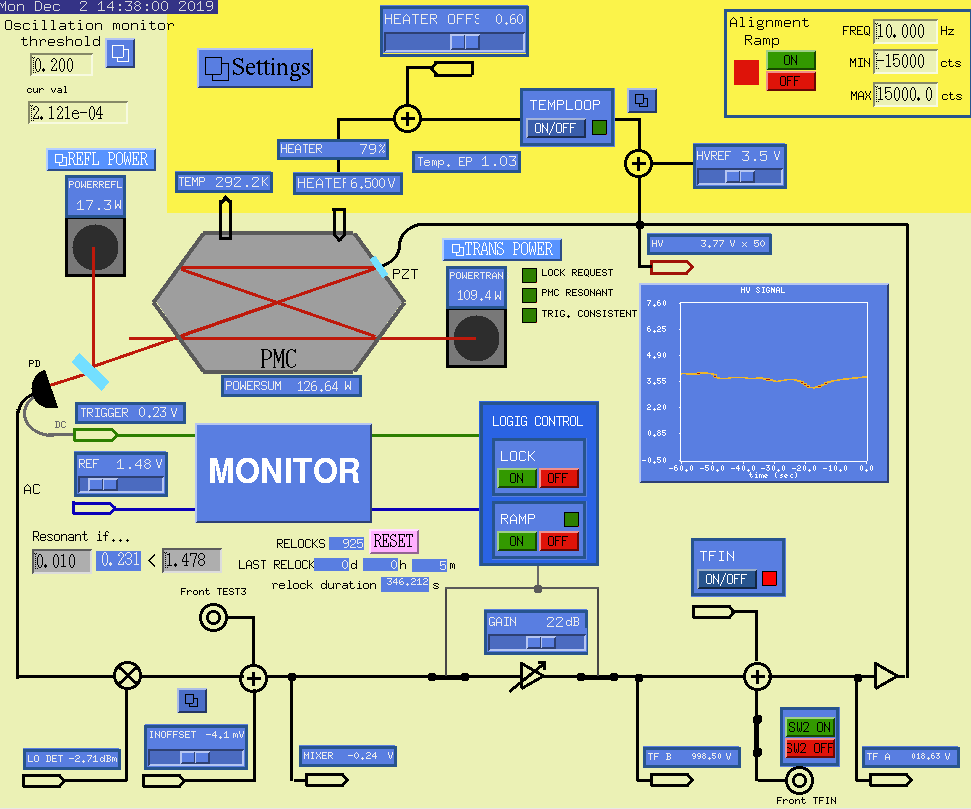
\includegraphics[width=0.9\linewidth]{Figures/medm_screen}
	\caption{This MEDM interface is used by operators of the interferometer to control and monitor the status of the PMC. Several inputs and outputs can be monitored simultaneously, and locking the PMC is reduced to simply pressing a button (\texttt{LOCK}). Most aspects of the locking servo can be adjusted with CDS, e.g. the \texttt{gain} slider adjusts the gain of the servo, thus operators have a large amount of freedom when they are trying to optimise the PMC's locking capabilities.}
	\label{fig:medmscreen}
\end{figure}
\par
CDS contains an array of analogue-to-digital converters (ADC) for accepting analogue signals and digital-to-analogue converters (DAC) for generating analogue outputs. An ADC measures a voltage, and the smallest voltage that it can measure is ultimately determined by the number of bits it uses. The smallest voltage measurable with the ADC corresponds to one count within CDS. 
\par
The Glasgow CDS uses ADCs with a voltage range of $\pm10\,\si{\volt}$, and the sample rate of the ADCs is 65\,kHz. The voltage is recorded as a signed 15 bit integer, so $2^{15}$ counts is equivalent to 10 Volts. Note that counts can exceed $2^{15}$ within the digital part of CDS. The digitised analogue input signals have a noise floor, and a measurement of this is shown in Figure~\ref{fig:mzchaptercdsnoise}. As digitally measured signals can be aliased if they exceed the bandwidth of the ADCs, signals that are measured with CDS are low passed at 9\,kHz with a third order filter. The noise of the Glasgow CDS analogue inputs is equivalent to an ADC with a 14 bit resolution.
\begin{figure}
	\centering
	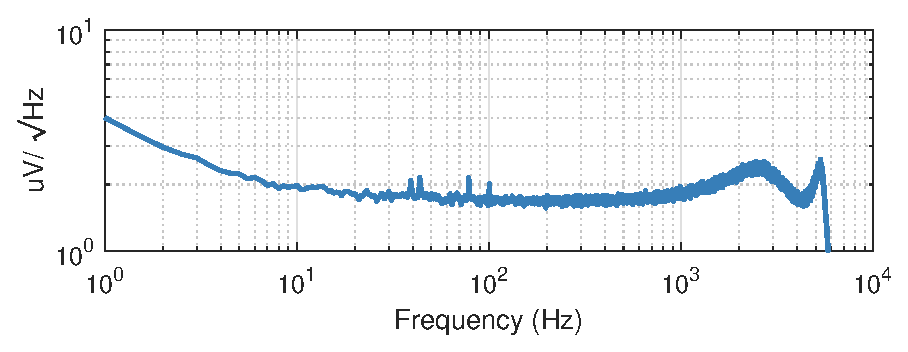
\includegraphics[width=1\linewidth]{Figures/MZ_chapter_CDS_noise}
	\caption{Noise floor of the digitised input signals recorded by the Glasgow CDS. This was converted into a voltage using $2^{15}$ counts per 10 Volts. The ripples above 1\,kHz arise due to the 3rd order low pass filter at 9\,kHz. Below $\sim10$\,Hz, the input noise rises as $1/f$.}
	\label{fig:mzchaptercdsnoise}
\end{figure}
